\documentclass[10pt,a4paper]{article}
\usepackage[utf8]{inputenc}
\usepackage[spanish]{babel}
\usepackage{amsmath}
\usepackage{amsfonts}
\usepackage{amssymb}
\usepackage{makeidx}
\usepackage{graphicx}
\usepackage[hidelinks]{hyperref}
\usepackage[left=2cm,right=2cm,top=2cm,bottom=2cm]{geometry}
\author{Ulises Isaac Reyes Alvarez\\Luis Osvaldo Cervantes Martinez\\4.B Ing. Mecatrónica\\Mtro. Carlos Enrique Morán Garabito\\"Sistemas Electrónicos de Interfaz"}
\title{Diagrama eléctrico de la interfaz de potencia}

\begin{document}
\maketitle
\begin{figure}[hbtp]
\centering

\includegraphics[scale=2]{Pictures/UPZMG.png}
\end{figure}

\newpage
\section{Introducción}
\subsection*{Objetivos}
\begin{itemize}
\item Armar un circuito electrico de interfaz de potencia
\item Obtener valor de entrada y salida en los circuitos
\item Lograr activar Transistor NPN TIP41C 
\end{itemize}

\subsection*{Marco téorico}
Un transistor (la contracción de transfer resistor, transferencia de resistencias) es un dispositivo semiconductor con tres terminales utilizando como amplificador e interruptor en el que una pequeña corriente o tensión aplicada a uno de los terminales controla o modula la corriente entre los otros dos terminales. Es el componente fundamental de la moderna electrónica, tanto digital como analógica.\\
En los circuitos digitales se usan como interruptores, y disposiciones especiales de transistores configuran las puertas lógicas, memorias RAM y otros dispositivos: en los circuitos analógicos se usa principalmente como amplificadores. 

\textbf{Condiciones de funcionbamiento}
Las condiciones normales de funcionamiento de un transistor NPN se dan cuando el diodo B-E se encuentra polarizado en directa y el diodo B-C se encuentra polarizado en inversa. En esta situación gran parte de los electrones que fluyen del emisor a la base consiguen atravesar ésta, debido a su poco grosor y débil dopado, y llegar al colector. 

El transistor posee tres zonas de funcionamiento:\\\

\textbf{1. Zona de saturación}\\
El diodo colector está polarizado directamente y esté transistor se comporta como una pequeña resistencia. En esta zona un aumento adicionar de la corriente de base no provoca un aumento de la corriente de colector, está depende exclusivamente de la tensión entre emisor y colector. El transistor se asemeja en su circuito emisor-colector a un interruptor cerrado. \\\

\textbf{2.Zona activa}\\
En este intervalo el transistor se comporta como una fuente de corriente, determinada por la corriente de base. A pequeños aumentos de la corriente de base corresponden grandes aumentos de la corriente de colector, de forma casi independiente de la tensión entre el emisor y el colector. Para trabajar en esta zona el diodo B-E ha de estar polarizado en directa, mientras que el diodo B-C, ha de estar polarizado en inversa. \\\

\textbf{3. Zona de corte}\\
El hecho de hacer nula la corriente de base, es equivalente a mantener el circuito base emisor abierto, en estas circunstancias la corriente de colector es prácticamente nula y por ello se puede considerar el transistor en su circuito C-E como un interruptor abierto. 

\begin{figure}[hbtp]
\centering
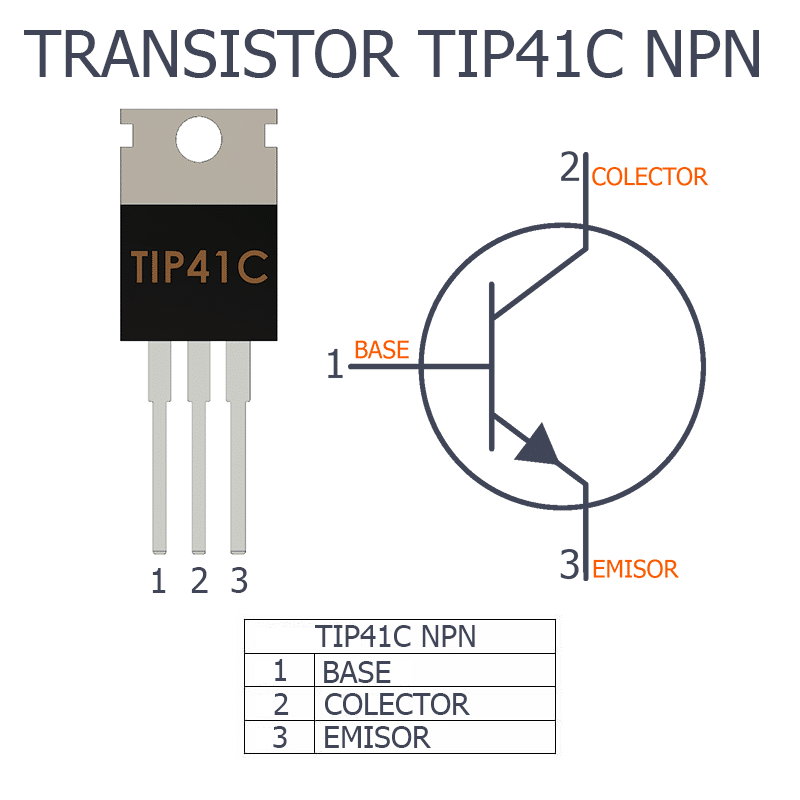
\includegraphics[scale=0.2]{Pictures/TIP41C.png}
\caption{Estructura del transistor TIP41C}
\end{figure}
\footnote{Universidad Politécnica de la Zona Metropolitana de Guadalajara}

\newpage
\section{Materiales y equipo}

\begin{itemize}
\item Protoboard
\item Cables para protoboard
\item Caimanes
\item Transistor NPN TIP41C / TIP31
\item Fuente de alimentación 1.5V, 9V  y 12V
\item Resitencias 47K$\Omega$, 1k$\Omega$ y 100$\Omega$
\item Capacitores 10$\mu$F, 100$\mu$F y 220$\mu$F
\item Bobinas 2.5mH hechas a mano o bobinas de transformador
\item LED's 
\item MOSFET TIP112
\item Potenciómetros 10k$\Omega$ y 5k$\Omega$
\item Amplificador operacional LM25
\end{itemize}
\footnote{Universidad Politécnica de la Zona Metropolitana de Guadalajara}

\newpage
\section{Desarrollo}
\textbf{1. Armar el siguiente circuito en protoboard}
\begin{figure}[hbtp]
\centering
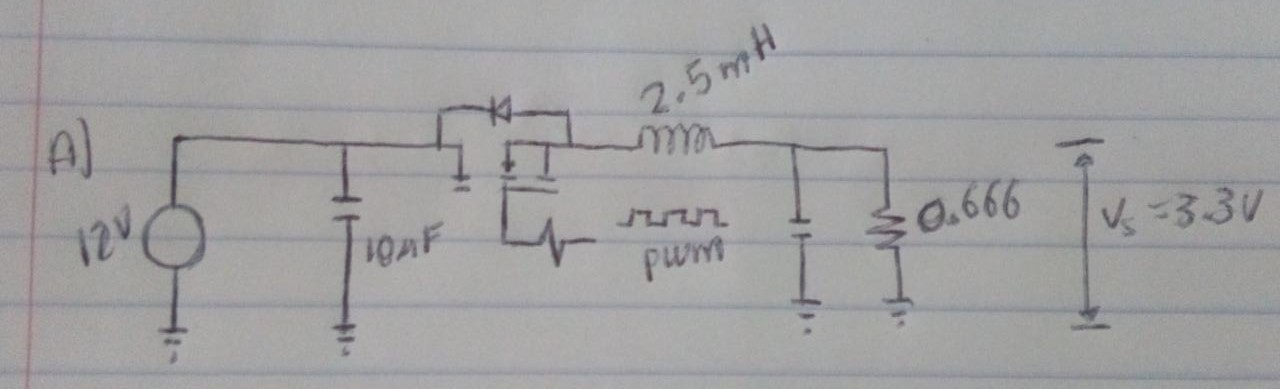
\includegraphics[scale=0.5]{Pictures/Circuito A.jpeg}
\caption{Circuito pwm}
\end{figure}

Primero que nada vamos a realizar el pwm, para interactuar con el circuito anterior y encender 2 LED's como se muestra a continuación: 
\begin{figure}[hbtp]
\centering
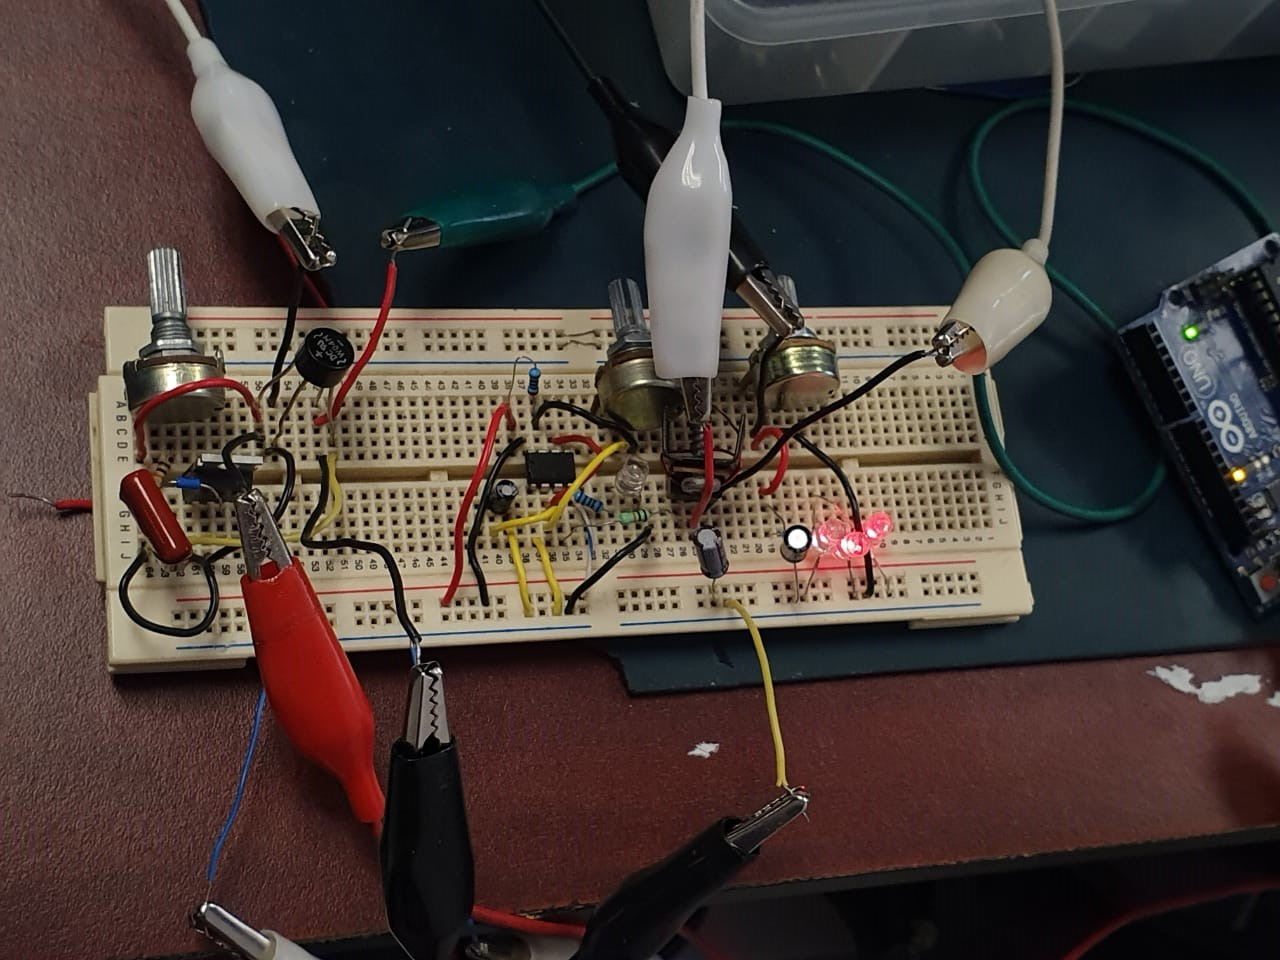
\includegraphics[scale=0.3]{Pictures/Pwm.jpeg}
\caption{Circuito armado pwm}
\end{figure}

Para esta parte del circuito hicimos una bobina con un tornillo y 3m de alambre de cobre magnetizado, enrollandolo en el tornillo y creando una bobina de 150 vueltas la cual la utilizamos para el circuito.\\
Observamos que al conectar las fuentes enciende un LED que indica que nuestro pwm esta funcionando, movemos el potenciometro y observamos que el LED comienza a parpadear, señalando que tenemos listo nuestro pwm listo para agregarle la siguiente parte.\\

Alimentamos la siguiente parte del circuito y lo que obtenemos es el encendido de 3 LED's, como se muestra a continuación: 

\footnote{Universidad Politécnica de la Zona Metropolitana de Guadalajara}

\newpage
\begin{figure}[hbtp]
\centering
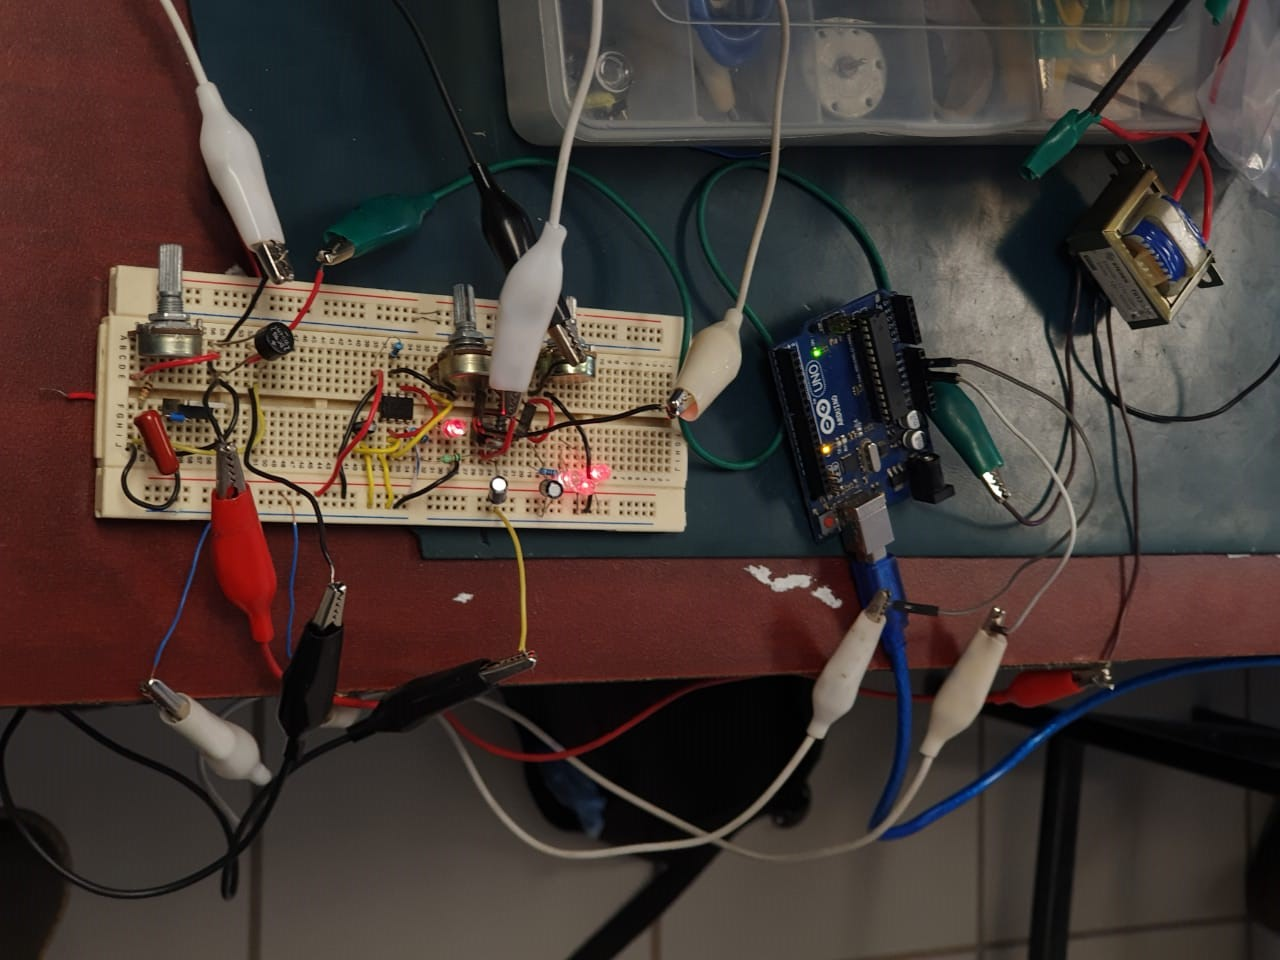
\includegraphics[scale=0.3]{Pictures/pwm2.jpeg}
\caption{Circuito pwm y circuito a)}
\end{figure}

Obtendremos como entrada 1V teniendo el potenciometro en apagado y como salida 4.65V para la alimentación de los LED's, haciendo funcionar mediante resistencia de 220$\Omega$.

\begin{figure}[hbtp]
\centering
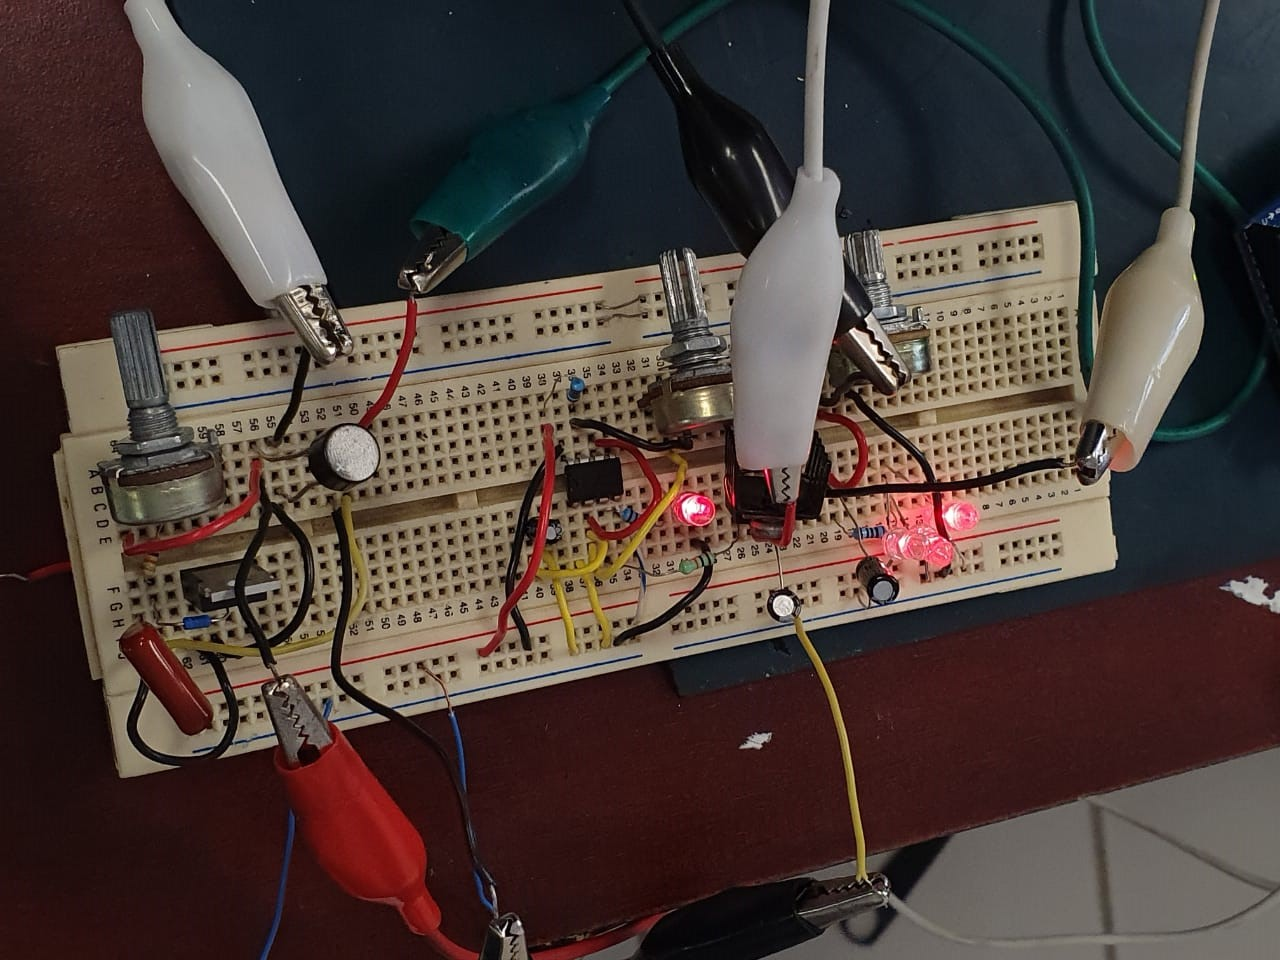
\includegraphics[scale=0.3]{Pictures/pwm1.jpeg}
\caption{Accionamiento del MOSFET TIP112}
\end{figure}
\footnote{Universidad Politécnica de la Zona Metropolitana de Guadalajara}

\newpage
\textbf{2. Vamos a armar el siguiente circuito para el accionamiento del Transistor TIP41C}

\begin{figure}[hbtp]
\centering
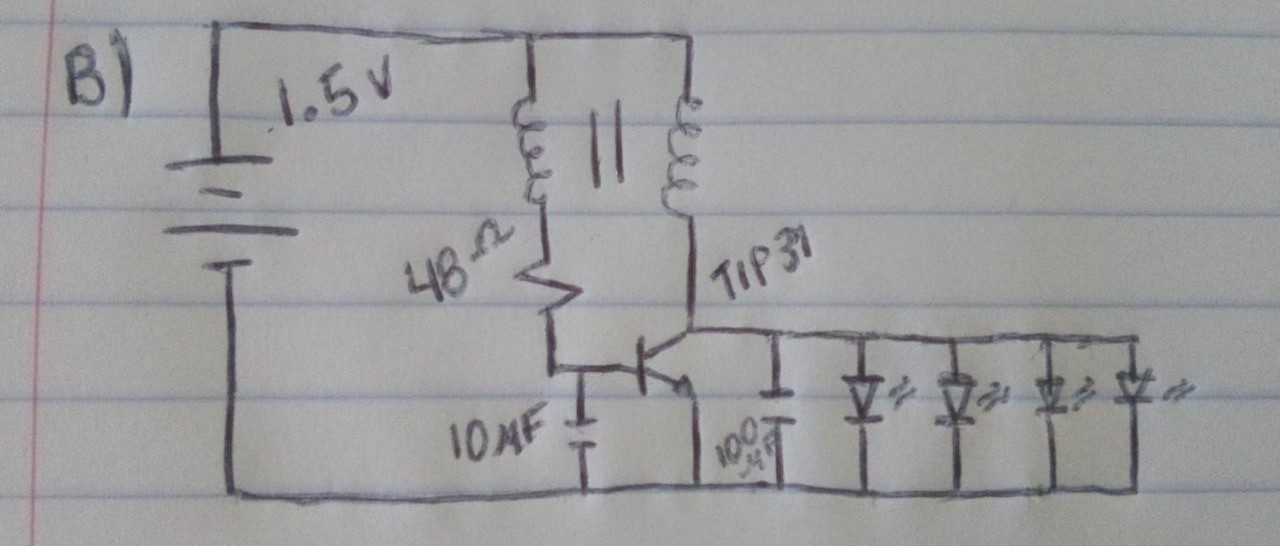
\includegraphics[scale=0.3]{Pictures/Circuito B.jpeg}
\caption{Circuito B activación TIP41C}
\end{figure}

Armamos el circuito b) en protoboard teniendo en cuenta que debemos colocar bien las patitas del Transistor tipo NPN para poder activar correctamente el TIP41C:
\begin{figure}[hbtp]
\centering
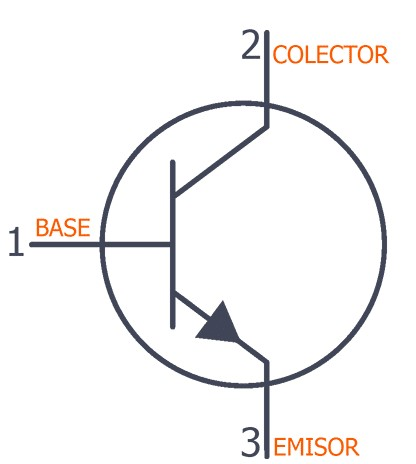
\includegraphics[scale=0.5]{Pictures/TIP41C.jpg}
\caption{Estructura TIP41C}
\end{figure}

El funcionamiento de este circuito es encender los 3 LED's mediante bobinas, en este caso mediante un transformador y la activación del TIP41C teniendo como resultado carga y descarga del capacitor, teniendo en la carga el encendido de los LED's y la descarga el apagado de los LED's:
\begin{figure}[hbtp]
\centering
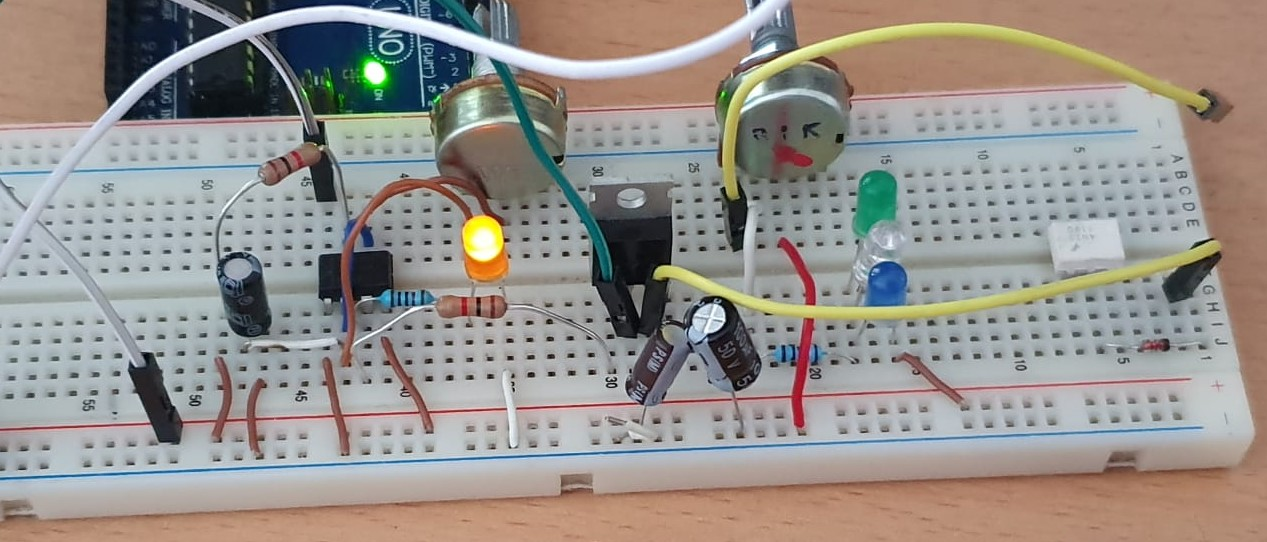
\includegraphics[scale=0.3]{Pictures/TIP.jpeg}
\caption{Activación TIP41C}
\end{figure}

\footnote{Universidad Politécnica de la Zona Metropolitana de Guadalajara}

\newpage
\section{Conclusiones}
\textbf{Luis Osvaldo Cervantes Martinez}\\
En esta práctica nos enfocamos en el uso de PWM, donde aplicamos nuestro conocimiento en practicas pasadas de los amplificadores operacionales, también nos pudimos percatar de que cuando la tensión de la entrada inversora es mayor que el de la entrada no inversora. Por otra parte y otro punto importante fue la activación del TIP41C, que básicamente es un amplificador de potencia el cual nos proporcionó la amplificación, dando un incremento de potencia.\\\\

\textbf{Ulises Isaac Reyes Alvarez}\\
En esta práctica aprendimos a desarrollar un pwm (pulse-width modulation) que es  una técnica en la que se modifica el ciclo de trabajo de una señal periódica (una senoidal o una cuadrada, por ejemplo), ya sea para transmitir información a través de un canal, en este caso la utilizamos para activar el TIP41C y encender LED's de 1.5V, con voltajes de entrada y salida. Aprendí a armar un circuito con un embobinado hecho por mi mismo, que si lo hacia mal, la práctica no funcionaría pero se logró. 

\footnote{Universidad Politécnica de la Zona Metropolitana de Guadalajara}

\newpage
\section{Referencias bibliográficas}
\url{https://es.slideshare.net/edicsson/transistor-tip-41-c}

\begin{figure}[hbtp]
\centering
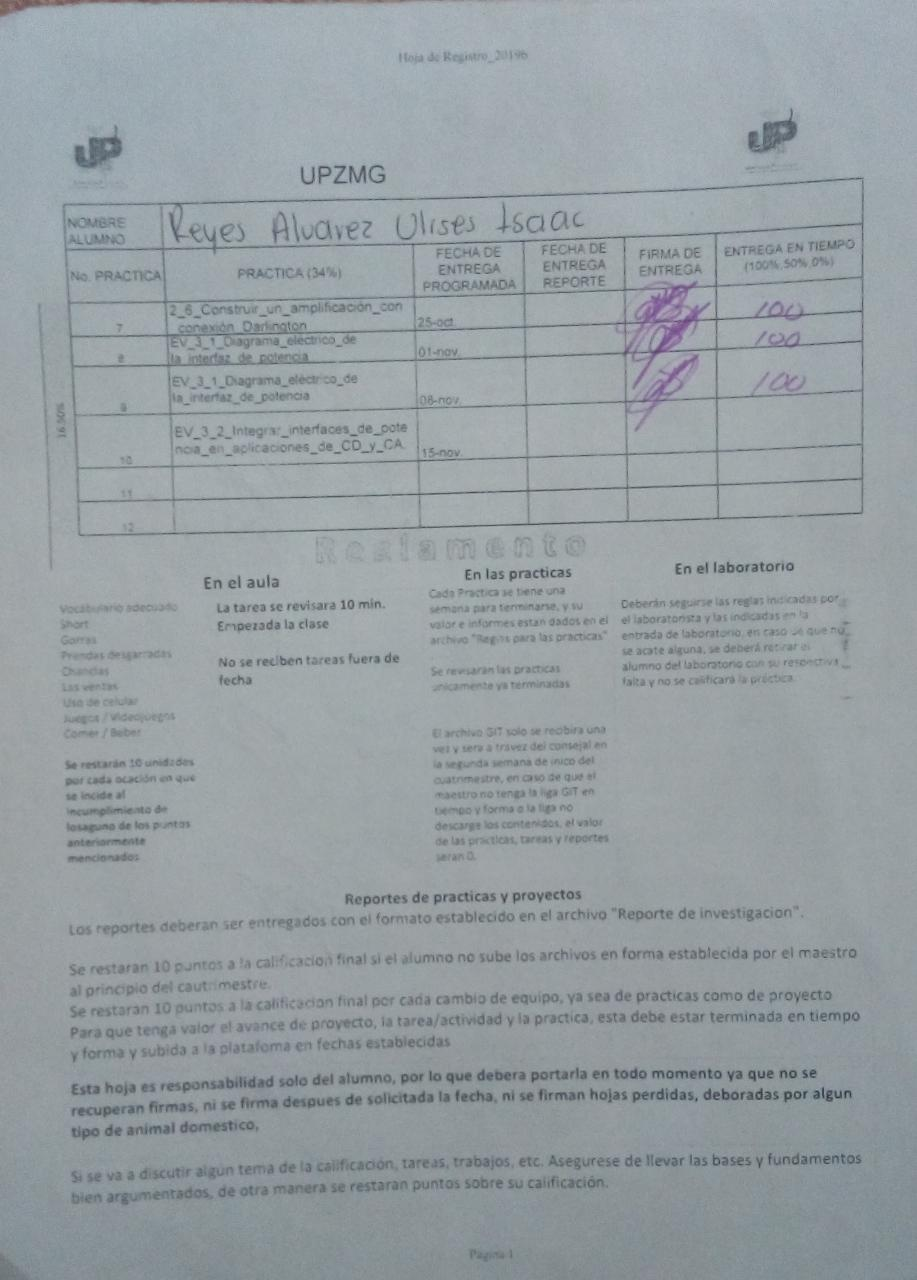
\includegraphics[scale=0.42]{Pictures/ULISES.png}
\caption{Ulises Isaac Reyes Alvarez  }
\end{figure}
\footnote{Universidad Politécnica de la Zona Metropolitana de Guadalajara}

\newpage
\begin{figure}[hbtp]
\centering
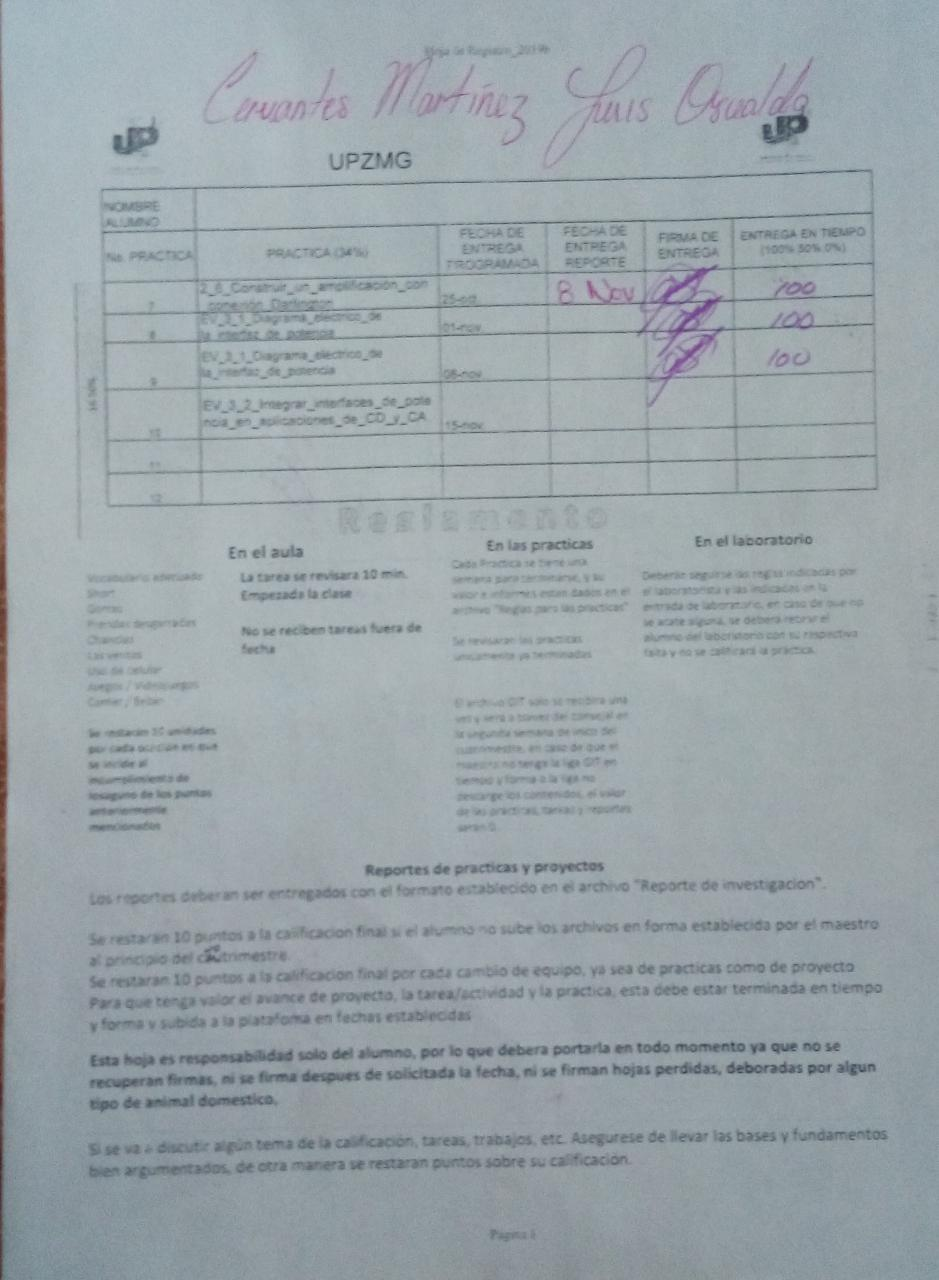
\includegraphics[scale=0.42]{Pictures/OSVALDO.png}
\caption{Luis Osvaldo Cervantes Martinez }
\end{figure}
\footnote{Universidad Politécnica de la Zona Metropolitana de Guadalajara}

\end{document}